\documentclass{beamer}
\usetheme{Luebeck}
\usecolortheme{beaver}
\setbeamertemplate{navigation symbols}{}

\usepackage{multimedia}
\usepackage{graphicx} 
\usepackage{animate}
\usepackage{multicol}
\usepackage{cite}
\usepackage[utf8]{inputenc}
\usepackage[ngerman]{babel}
\usepackage{tikz}
\usetikzlibrary{calc}

\definecolor{pbfill}{HTML}{FF6960}% filling color for the progress bar
\definecolor{pbbg}{HTML}{575757}% background color for the progress bar

\makeatletter
\newcommand\progressbar@progressbar{} % the progress bar
\newcount\progressbar@tmpcounta% auxiliary counter
\newcount\progressbar@tmpcountb% auxiliary counter
\newdimen\progressbar@pbht %progressbar height
\newdimen\progressbar@pbwd %progressbar width
\newdimen\progressbar@tmpdim % auxiliary dimension

\progressbar@pbwd=\paperwidth
\progressbar@pbht=0.5ex
\newcommand\progressbar@ffn{1}% Anzahl frames für Titelseite und 


% add page numbering
\expandafter\def\expandafter\insertshorttitle\expandafter{%
	\insertshorttitle\hfill%
	\hspace{40px}\insertframenumber\,/\,\inserttotalframenumber}

% the progress bar
\def\progressbar@progressbar{%
	\ifnum\insertframenumber>\progressbar@ffn
	
	\progressbar@tmpcounta=\insertframenumber
	\advance\progressbar@tmpcounta by -\progressbar@ffn
	\progressbar@tmpcountb=\inserttotalframenumber
	\advance\progressbar@tmpcountb by -\progressbar@ffn
	\progressbar@tmpdim=\progressbar@pbwd
	\multiply\progressbar@tmpdim by \progressbar@tmpcounta
	\divide\progressbar@tmpdim by \progressbar@tmpcountb
	
	\begin{tikzpicture}
		
	%%\shade[top color=pbbg!20,bottom color=pbbg!20,middle color=pbbg!20]
	\path[fill=pbbg!20]
	(0pt, 0pt) rectangle ++ (\progressbar@pbwd, \progressbar@pbht);
	
	%%\shade[draw=pbfill,top color=pbfill!50,bottom color=pbfill!50,middle color=pbfill] 
	\path[fill=pbfill!70]
	(0pt, 0pt) rectangle ++ (\progressbar@tmpdim, \progressbar@pbht);
	
	\end{tikzpicture}%
	\fi%
}

\addtobeamertemplate{footline}
{%
	\begin{beamercolorbox}[wd=\paperwidth,ht=3ex,center,dp=0ex]{white}%
		\progressbar@progressbar%
	\end{beamercolorbox}%
}{}
\makeatother
%#####


\title{Fouriertransformation -- Abtasttheorem}
\author{Steffen Walter (1145690) \ Marvin Gaube (4670273)}
\institute{Duale Hochschule Baden-Württemberg -- Stuttgart\newline Vorlesung: Digitale Bildverarbeitung}
\centering
\date{16. April 2020}
\begin{document}
	\maketitle
	\begin{frame}{Agenda}
		\begin{enumerate}
			\item Theoretische Grundlagen
			\begin{itemize}
				\item Abtastung
				\item 1D Aliasing-Effekt
				\item 1D Abtasttheorem
				\item 2D Aliasing-Effekt
				\item 2D Abtasttheorem
			\end{itemize}
			\item Realisierung
			\begin{itemize}
				\item MATLAB: FFT2
				\item Implementierung in MATLAB
				\item Demo
			\end{itemize}
			\item Fazit
		\end{enumerate}
	\end{frame}

	
	\begin{frame}{Abtastung}
	\section{Theoretische Grundlagen}
	%	Die Digitalisierung eines kontinuierlichen Bildes bedeutet einen enor-
	%	men Datenverlust, da wir die kontinuierliche Grauwertinformation auf
	%	eine Funktion auf einem Raster von Punkten reduzieren. Es stellt sich al-
	%	so die entscheidende Frage, unter welchen Bedingungen wir sicherstellen
	%	können, dass die Abtastpunkte das kontinuierliche Bild realitätsgetreu,
	%	also ohne Informationsverlust, wiedergeben. Zusätzlich interessiert uns,
	%	wie sich ein kontinuierliches Bild aus den Abtastpunkten rekonstruieren
	%	lässt.
	\begin{itemize}
		\item Abtastung bedeutet, dass nur die Information an den Gitterpunkten erhalten bleibt
		\item Multiplikation mit einer Funktion, die nur an den Gitterpunkten ungleich null ist
		\item Diese Operation lässt sich durchführen, indem wir die Bildfunktion $g(x)$ mit einer Funktion multiplizieren, welche die Summe der an den Gitterpunkten $r_{m,n}$ sitzenden $\delta$-Funktionen darstellt
		\item Die Funktion wird in der Literatur oft als Nagelbrettfunktion oder 2D-$\delta$-Kamm bezeichnet
	\end{itemize}	
	\end{frame}
	\begin{frame}{Abtastung}
	\begin{figure}
		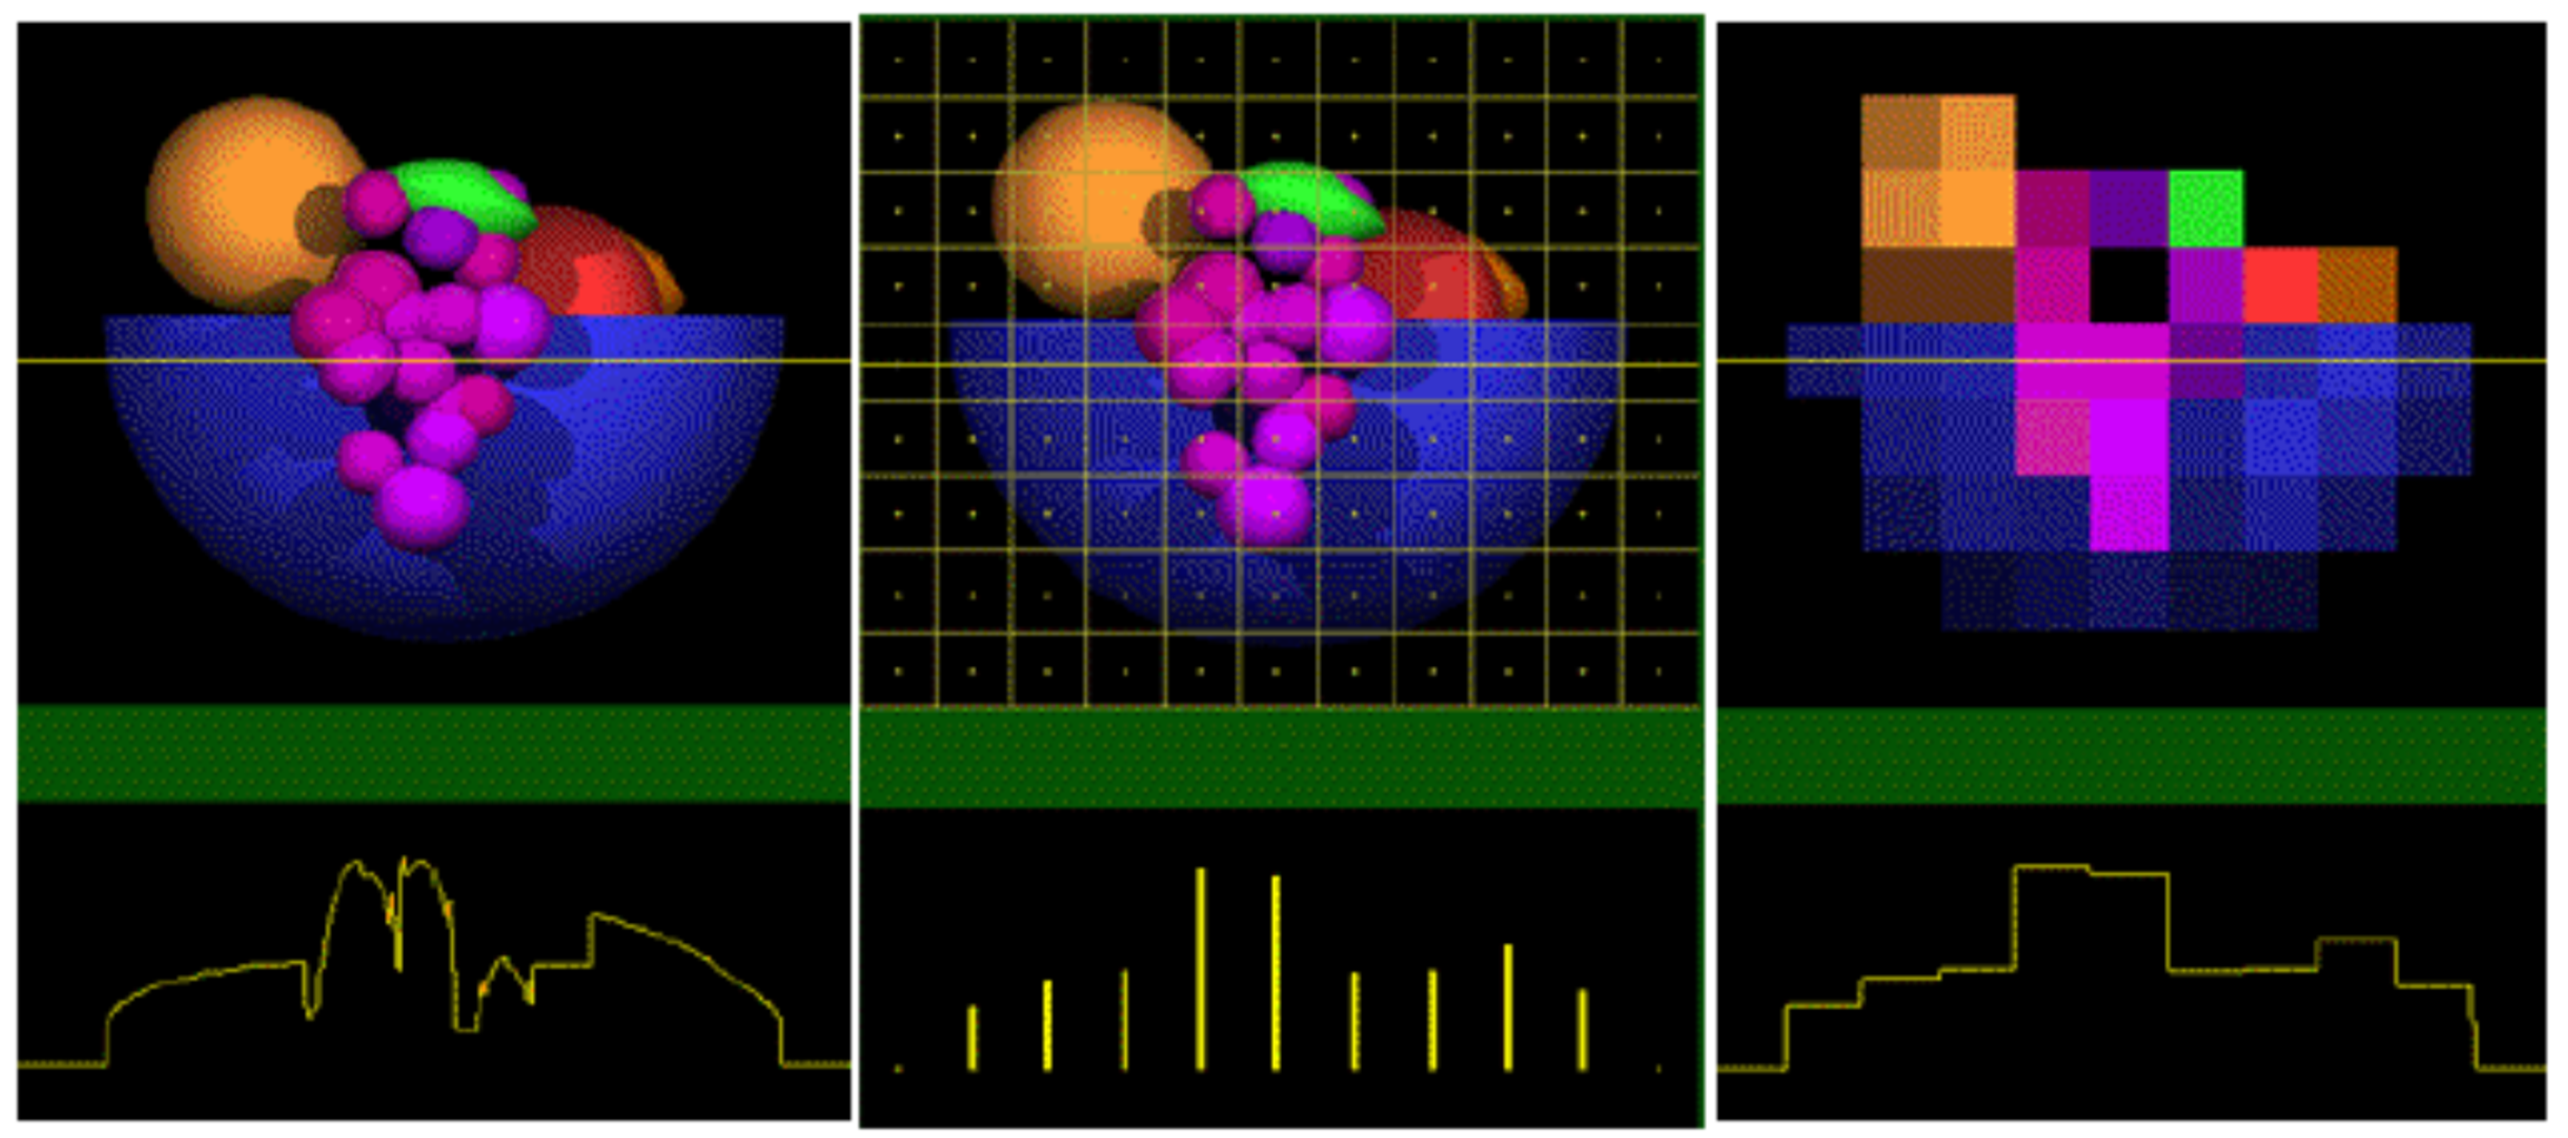
\includegraphics[width=1.3\textheight]{sampling.pdf}
		\caption{Beispiel Abtastung Quelle\cite{mit}}
	\end{figure}
	\end{frame}

	\begin{frame}{Abtastung}
	\begin{multicols}{2}
		\begin{itemize}
			\small\item Eine dichte Abtastung im x-Raum führt zu einem weiten Gitter im k-Raum und umgekehrt. Damit führt die Abtastung zu einer Wiederholung des Bildspektrums an jedem Gittervektor im Fourierraum.
			\item Die Abtastung führt zu einer Reduktion der Auflösung, das heißt, dass Strukturen von der Größe der Abtastschrittweite oder kleiner verloren gehen.
		\end{itemize}
		\begin{figure}
			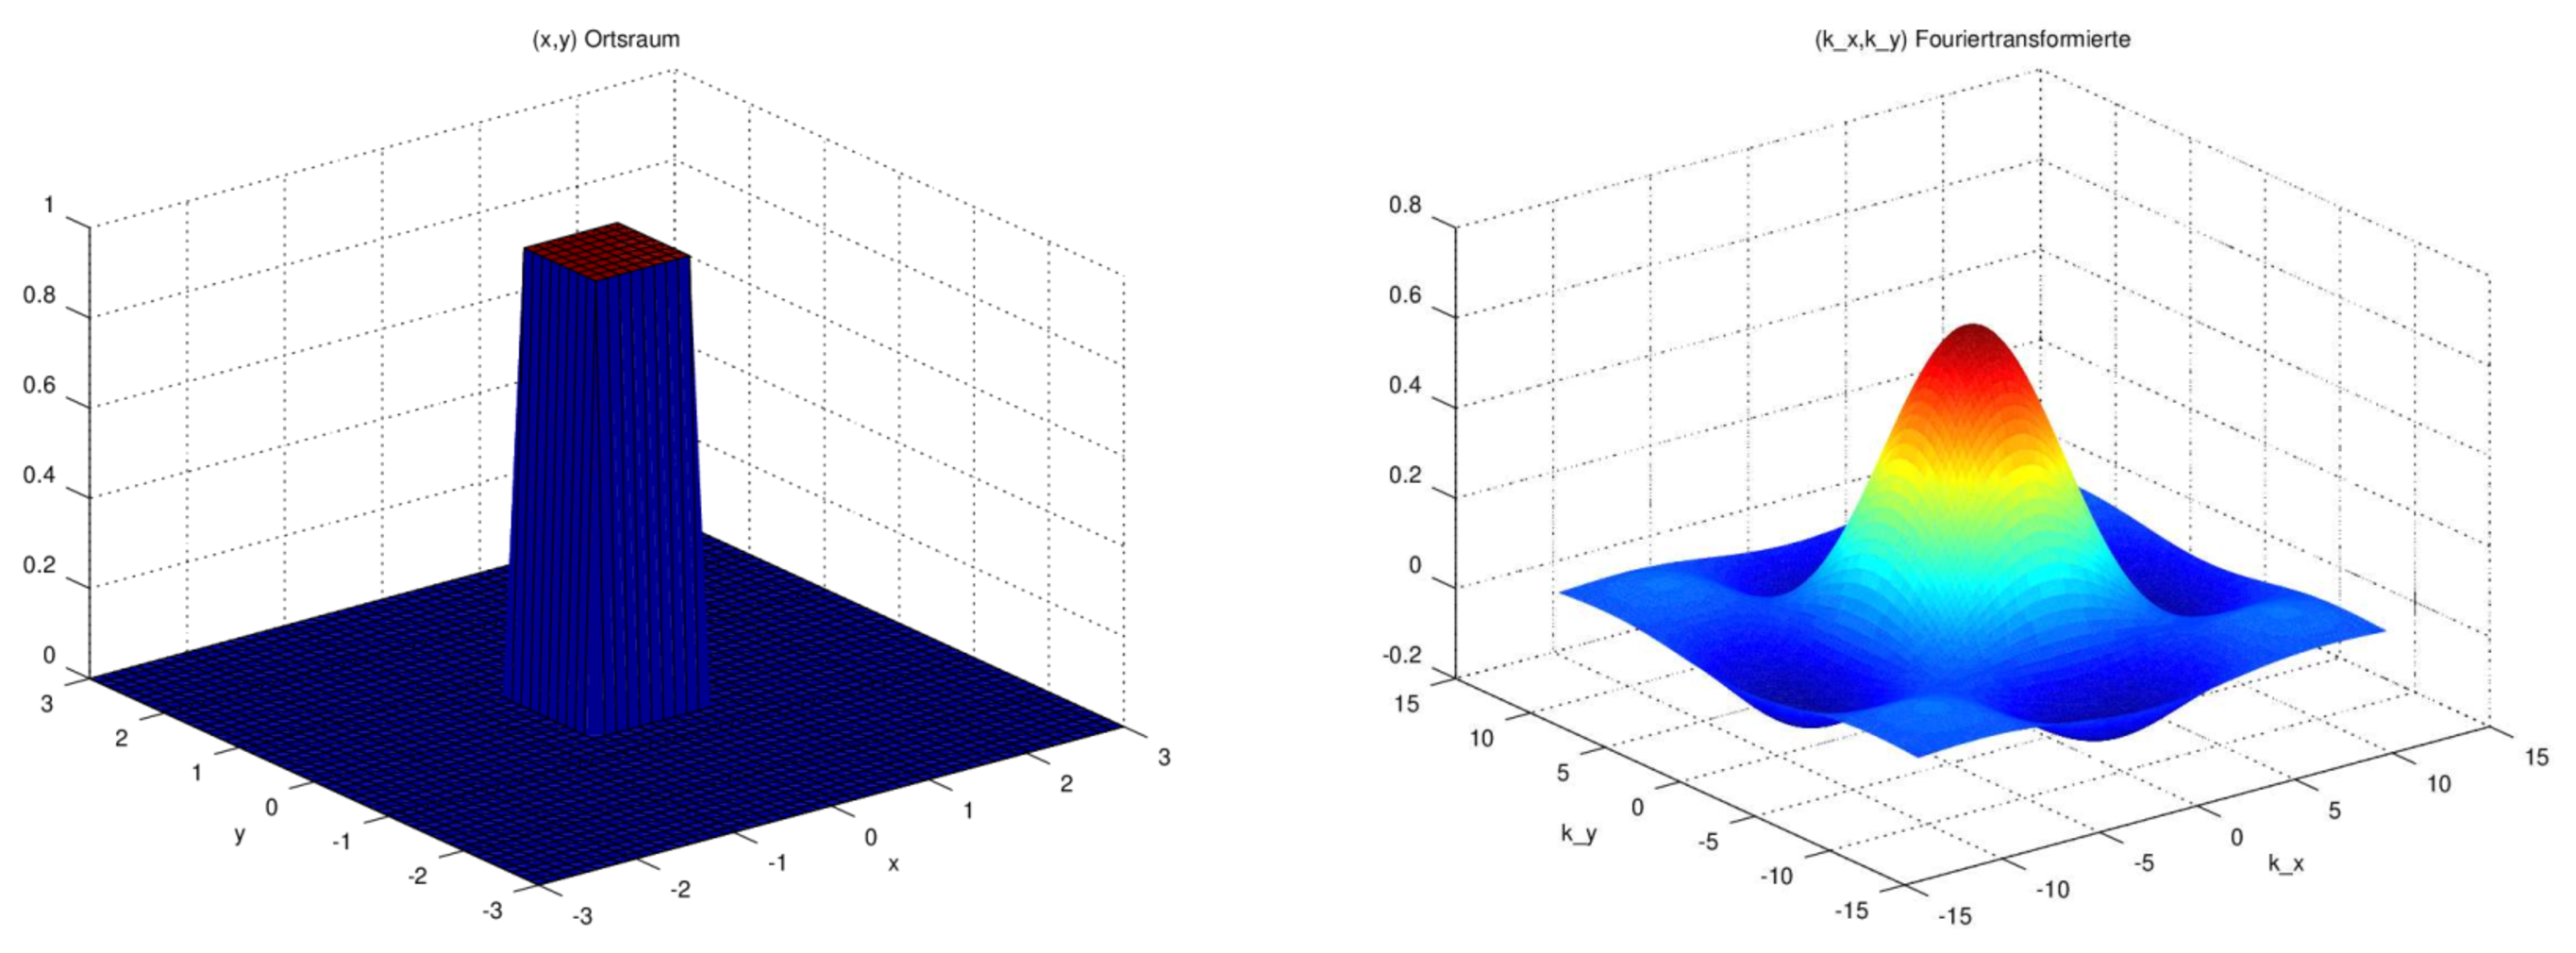
\includegraphics[width=0.6\textheight]{abtast1.pdf}
			\caption{\tiny Fouriertransformierte kleines Quadrat Quelle\cite{fuchs}}
		\end{figure}
		\begin{figure}
			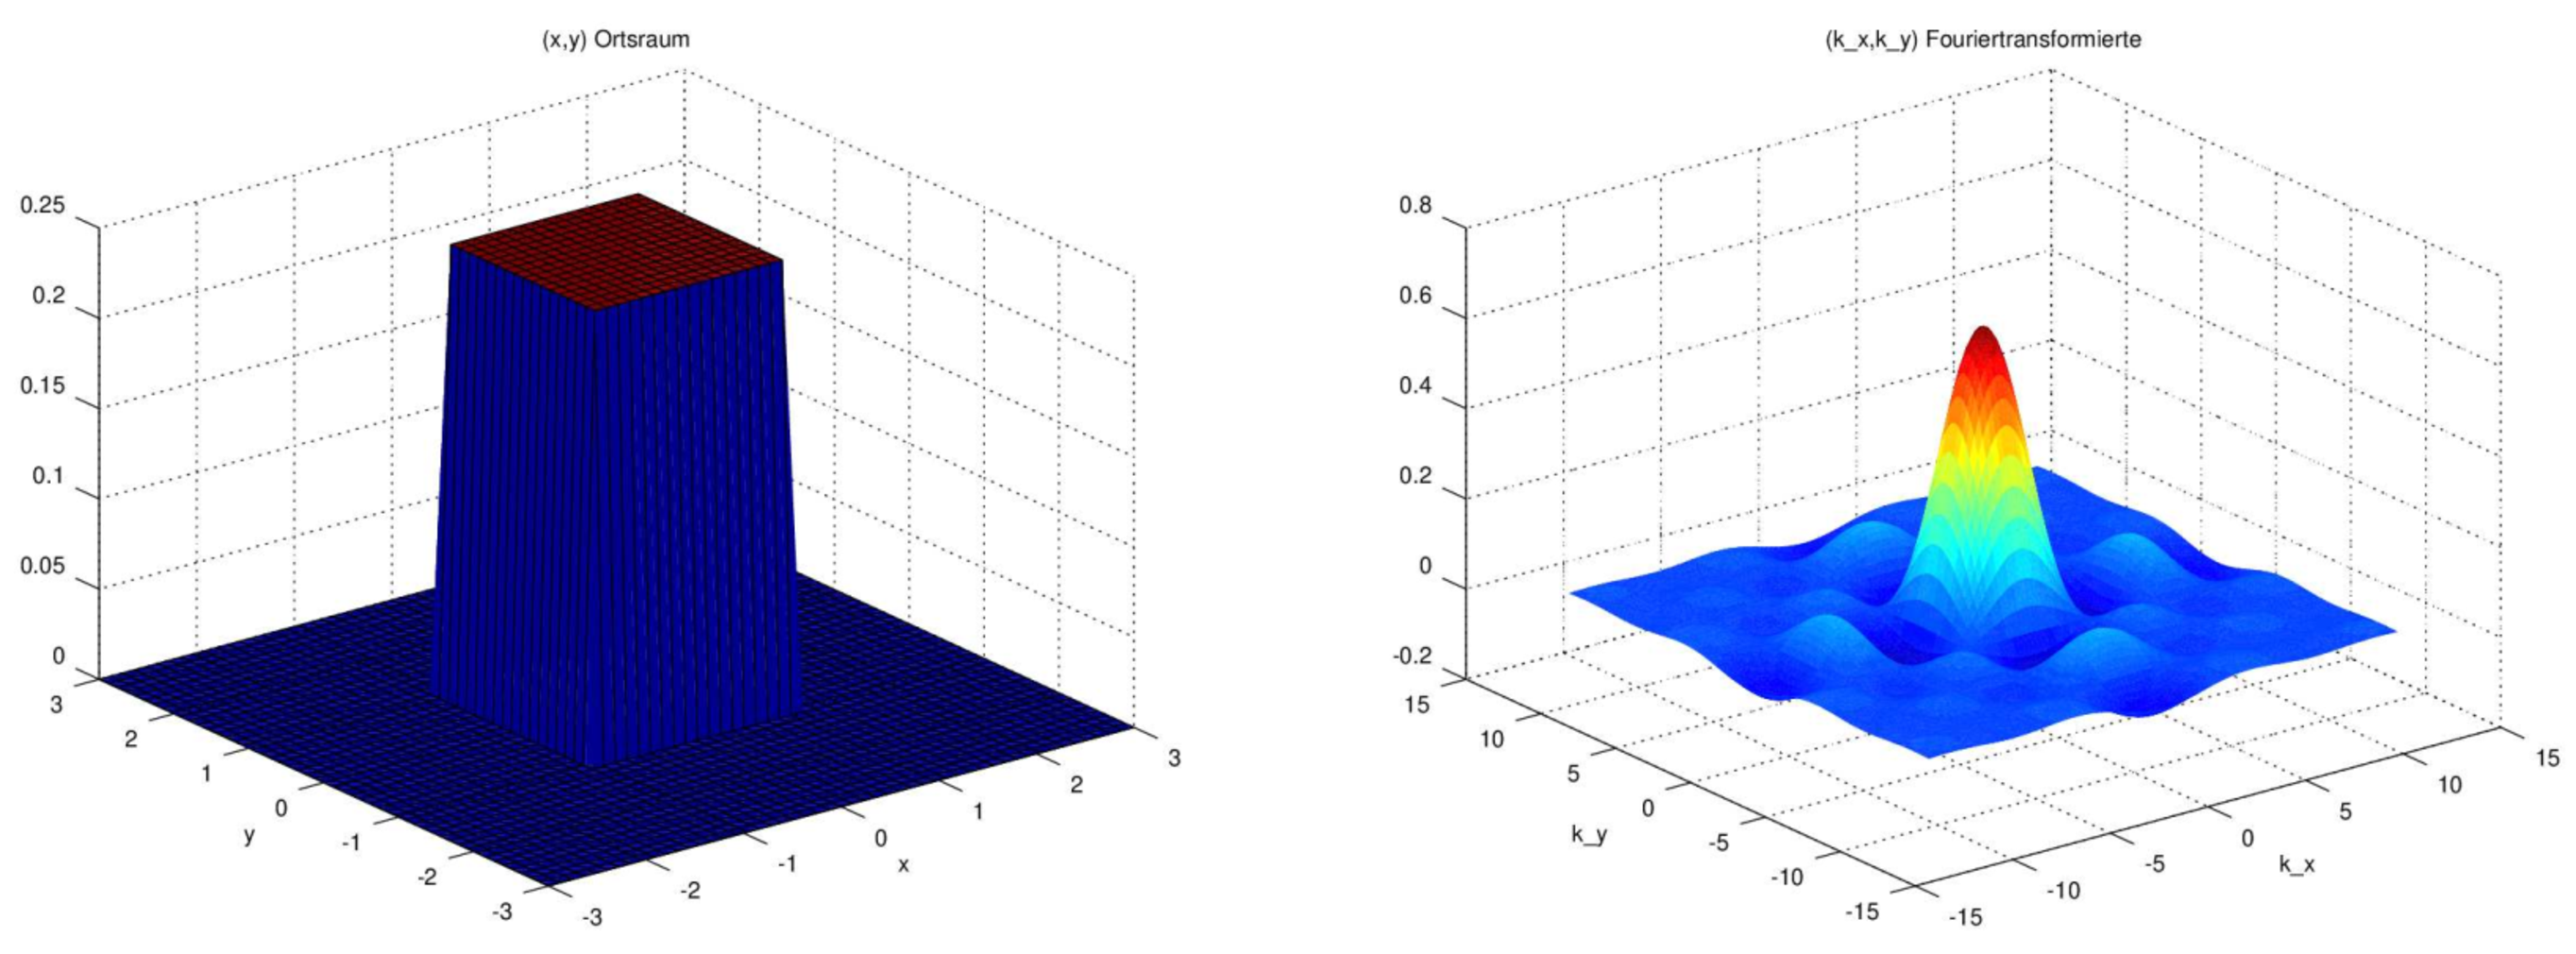
\includegraphics[width=0.6\textheight]{abtast2.pdf}
			\caption{\tiny Fouriertransformierte großes Quadrat Quelle\cite{fuchs}}
		\end{figure}
	\end{multicols}
	\end{frame}

	\begin{frame}{1D Aliasing-Effekt}
	\begin{block}{Beschreibung}
		\small Bei der Abtastung eines Signals mit einer Abtastfrequenz etwas kleiner als eine im Signal vorkommende Wellenlänge kann es zum Aliasing-Effekt kommen. Aus dem hochfrequenten Signal wird ein nicht vorhandenes niederfrequenteres Signal erkannt. Diese erkannte Frequenz wird Aliasfrequenz genannt 
	\end{block}
	
	\begin{figure}
		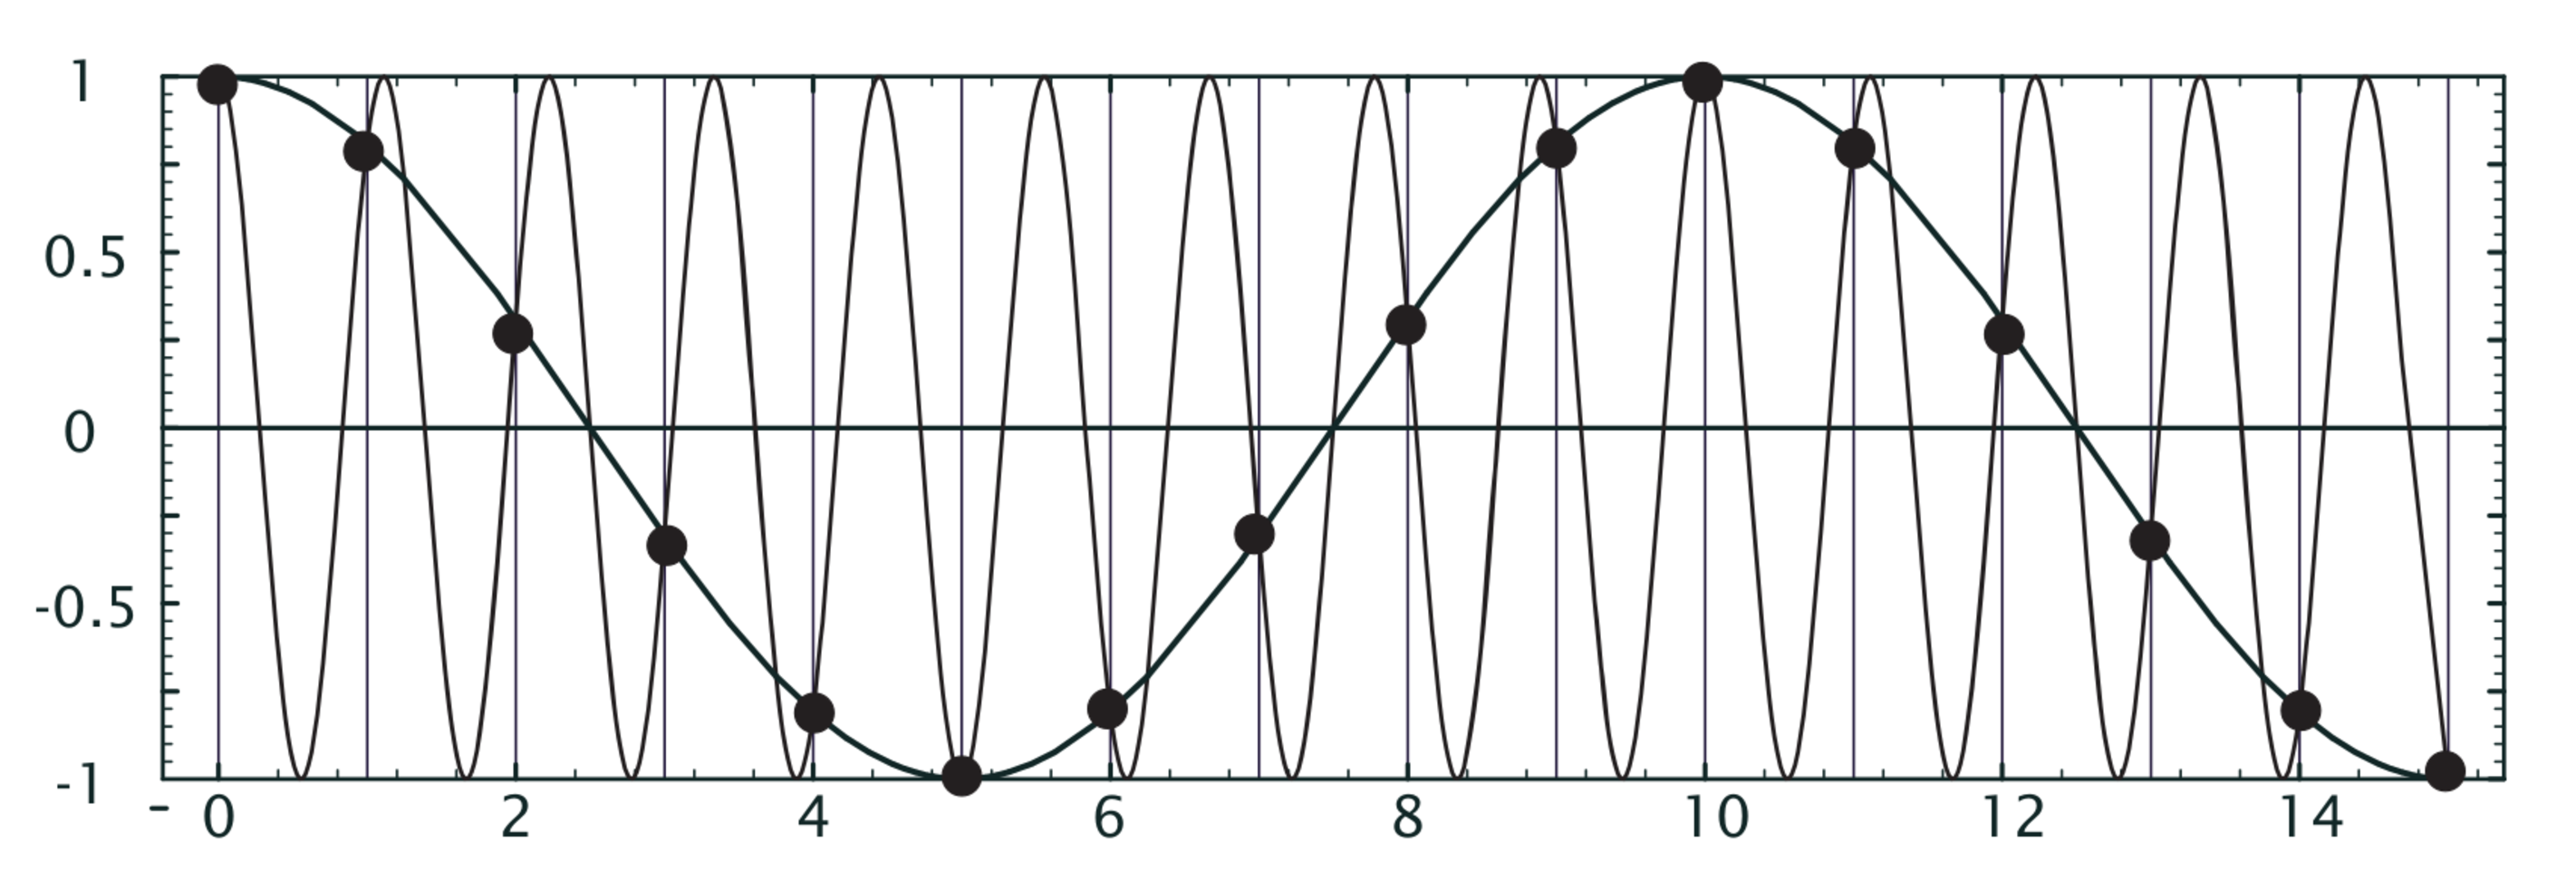
\includegraphics[width=\textheight]{antialiasing.pdf}
		\caption{\footnotesize Veranschaulichung des Aliasing-Effektes. Quelle\cite{bildverarbeitung}}
	\end{figure}
	
	\end{frame}

	\begin{frame}{1D Abtasttheorem}
	\begin{block}{Beschreibung}
		Das Abtasttheorem formuliert die Bedingung, welche nötig ist um eine Verfälschung des Signals bei der Abtastung zu vermeiden:
	\end{block}
	\begin{multicols}{2}
		
	
	\begin{itemize}
		\item Aus Abbildung ergibt sich $(f_p-f_g)-f_g \ge 0$
		\item Daraus lässt sich folgendes Ableiten: $f_p \ge 2f_g$
		\item $f_p$ ist hierbei die Abtastfrequenz 
	\end{itemize}
	
	\begin{figure}
		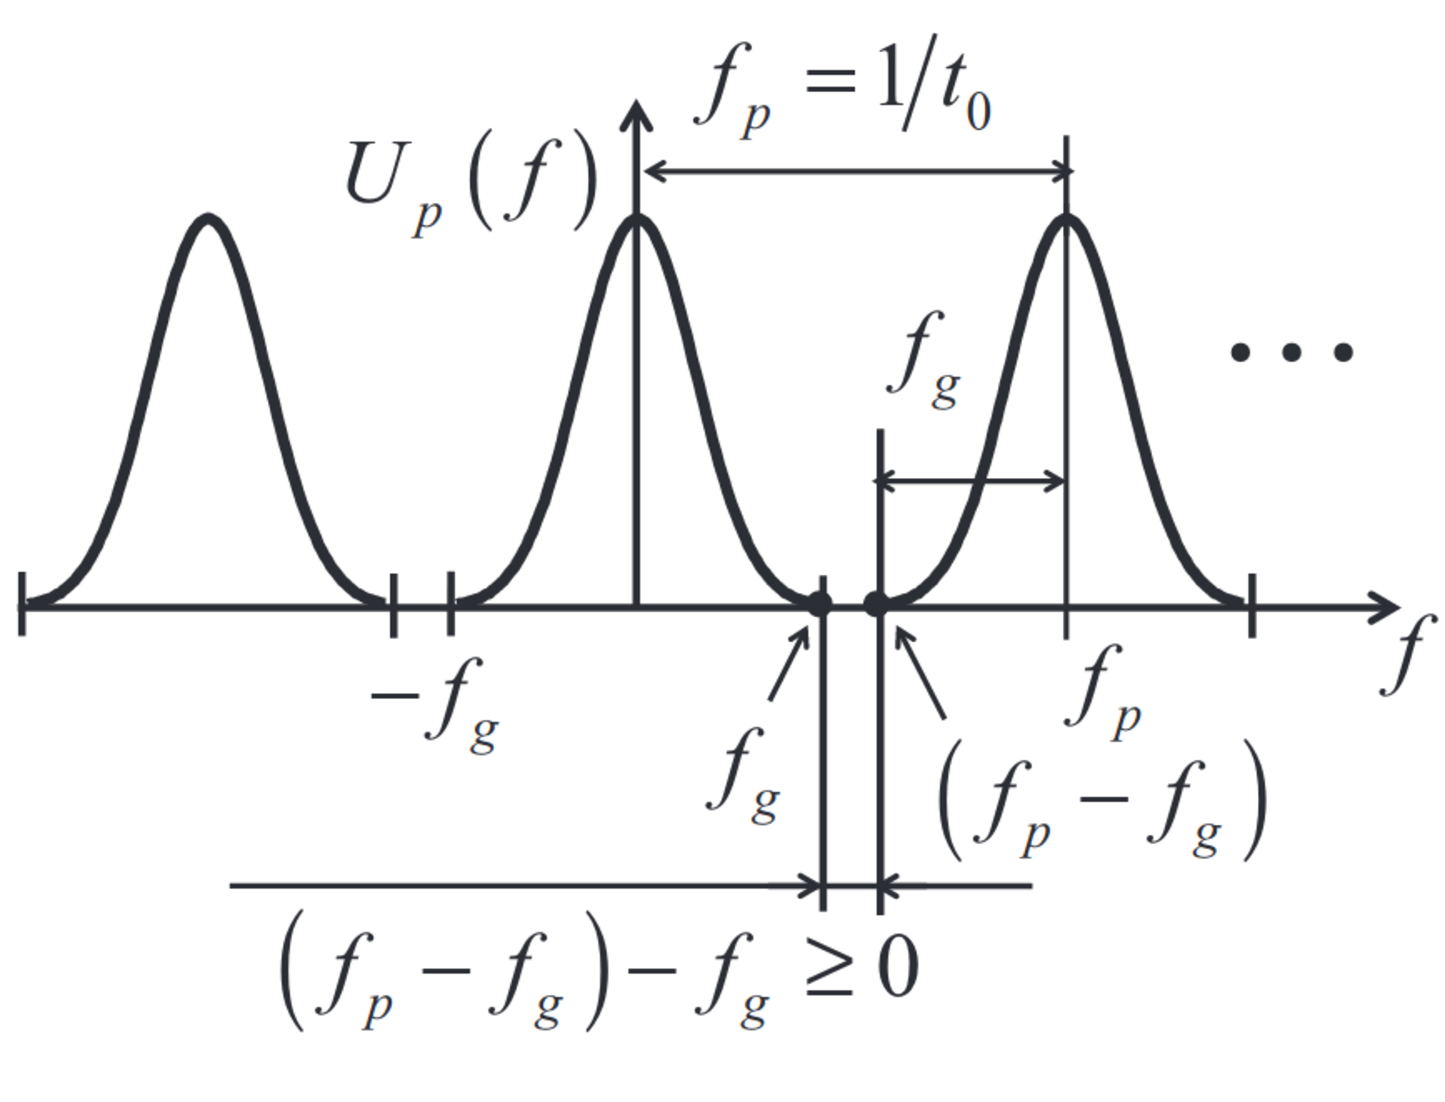
\includegraphics[width=0.58\textheight]{abtasttheorem.pdf}
		\caption{\footnotesize Bedingungen Abtasttheorem. Quelle\cite{lange}}
	\end{figure}
	\end{multicols}
	\end{frame}

	\begin{frame}{2D Aliasing-Effekt}
	\framesubtitle{Moiré-Effekt}
	\begin{figure}
		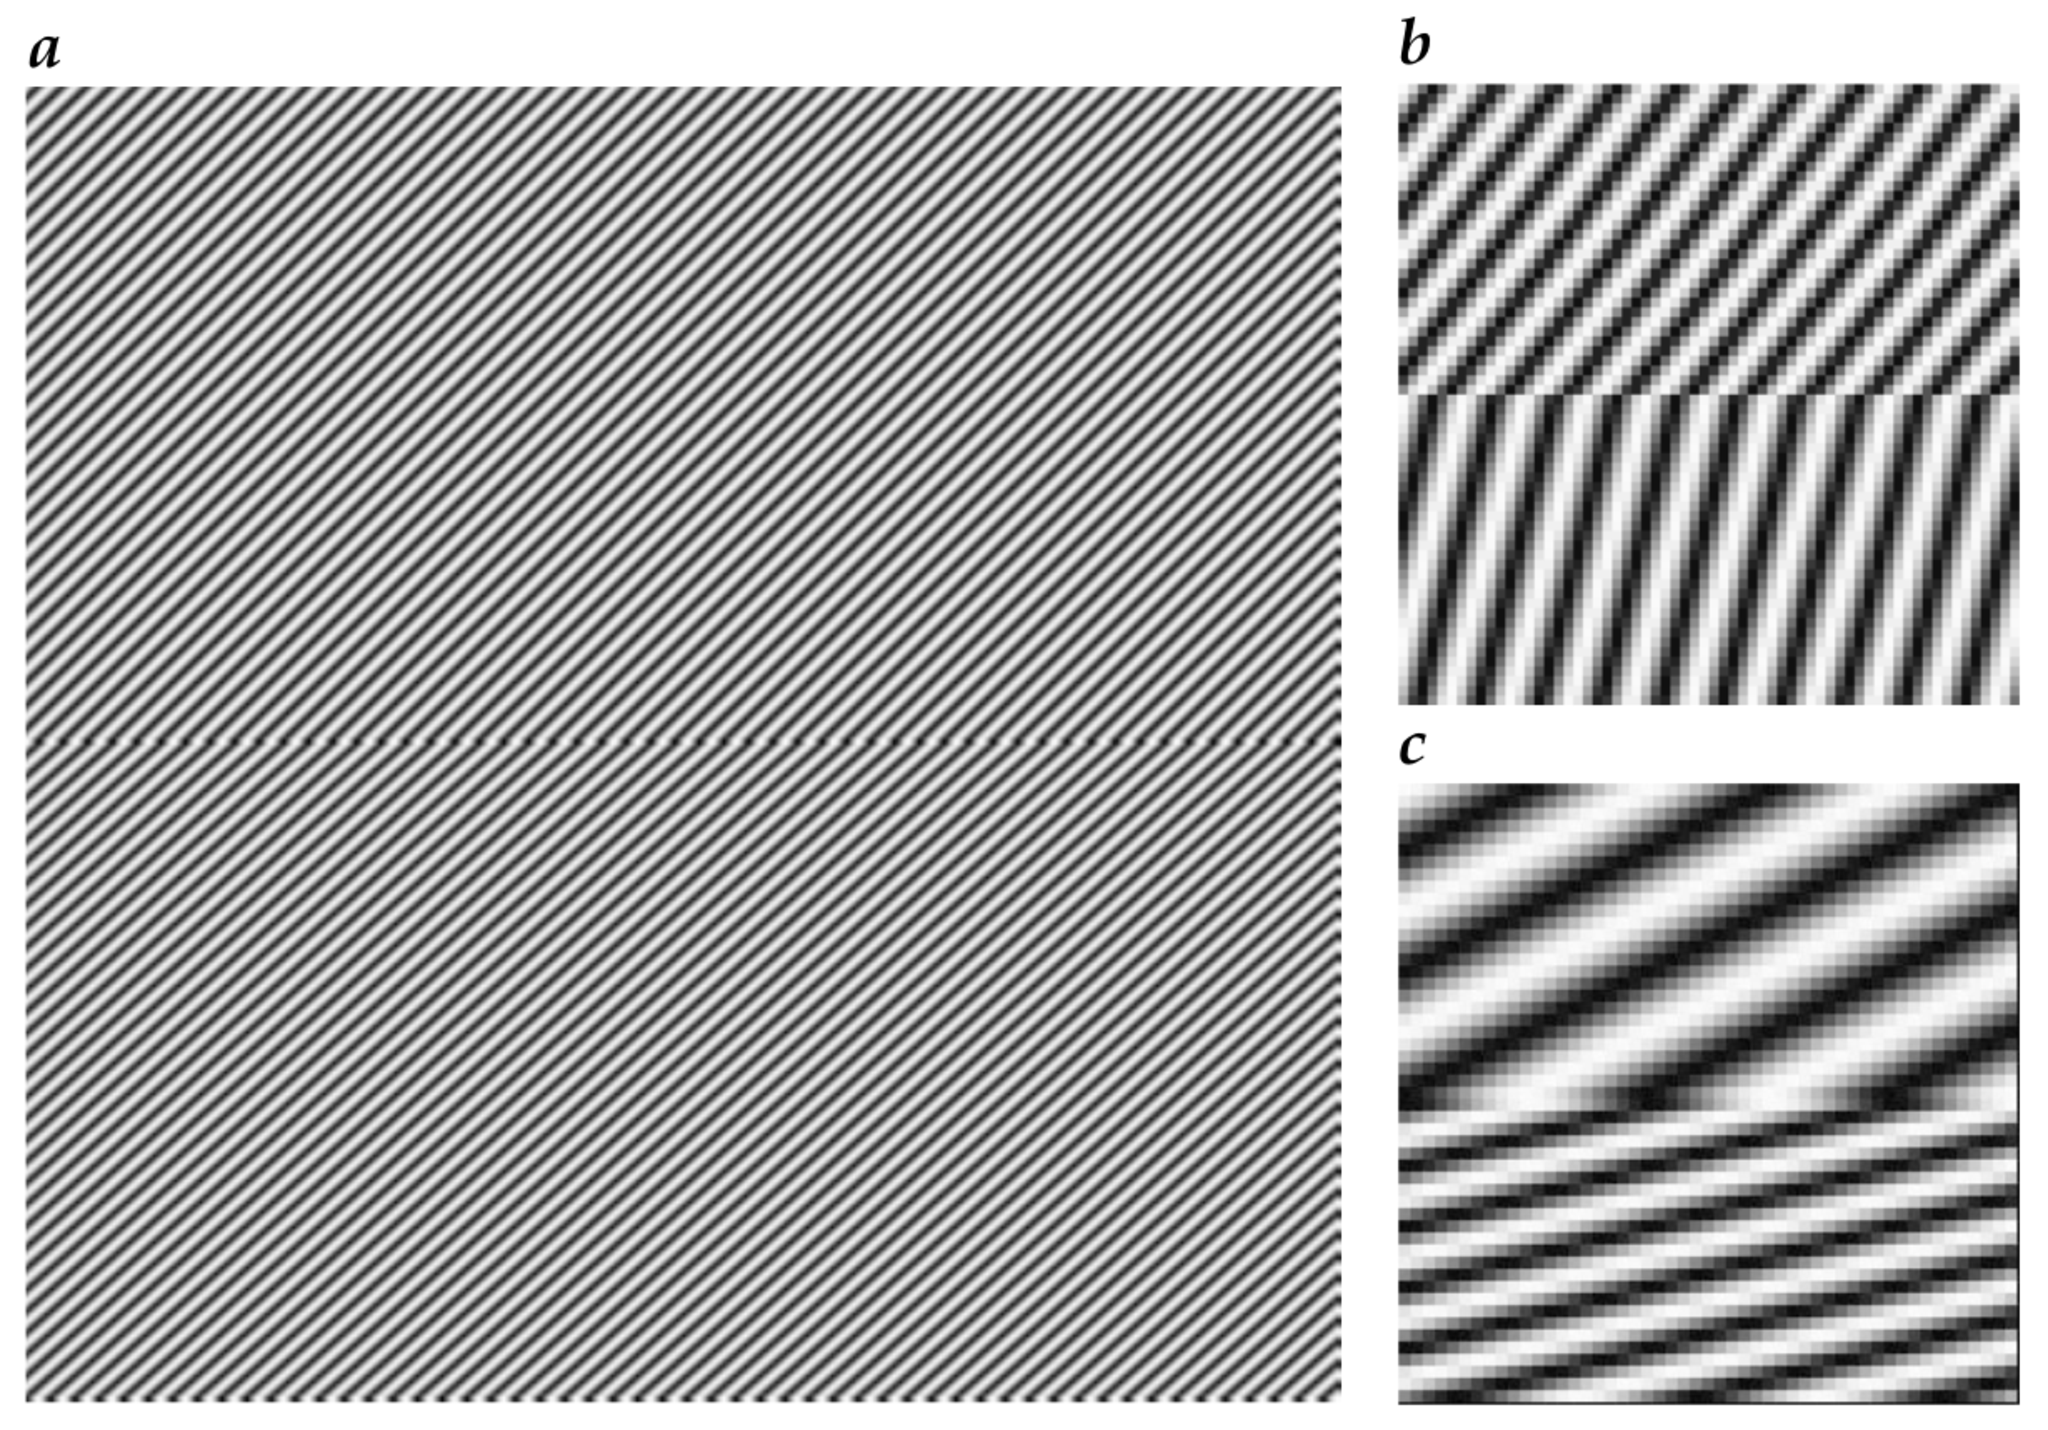
\includegraphics[width=0.7\textheight]{moire.pdf}
		\movie[height=3.5cm, width=5cm, poster, loop]{}{moire.mpg}
		\caption{\footnotesize Der Moiré-Effekt: \textbf{a} Originalbild mit zwei periodischen Mustern (oben $\hat{k} = [0.21, 0.22]^T$ , unten $\hat{k} = [0.21, 0.24]^T$ ). \textbf{b} Jeder vierte und \textbf{c} jeder fünfte Punkt in jeder	Richtung abgetastet. Quelle 1 (links)\cite{bildverarbeitung} Quelle 2 (rechts) \href{https://upload.wikimedia.org/wikipedia/en/4/42/Moir\%C3\%A9.gif}{Internet-Link}}
	\end{figure}
	\end{frame}

	\begin{frame}{Exkurs: Abtastung und Fouriertransformation}
		\begin{figure}
			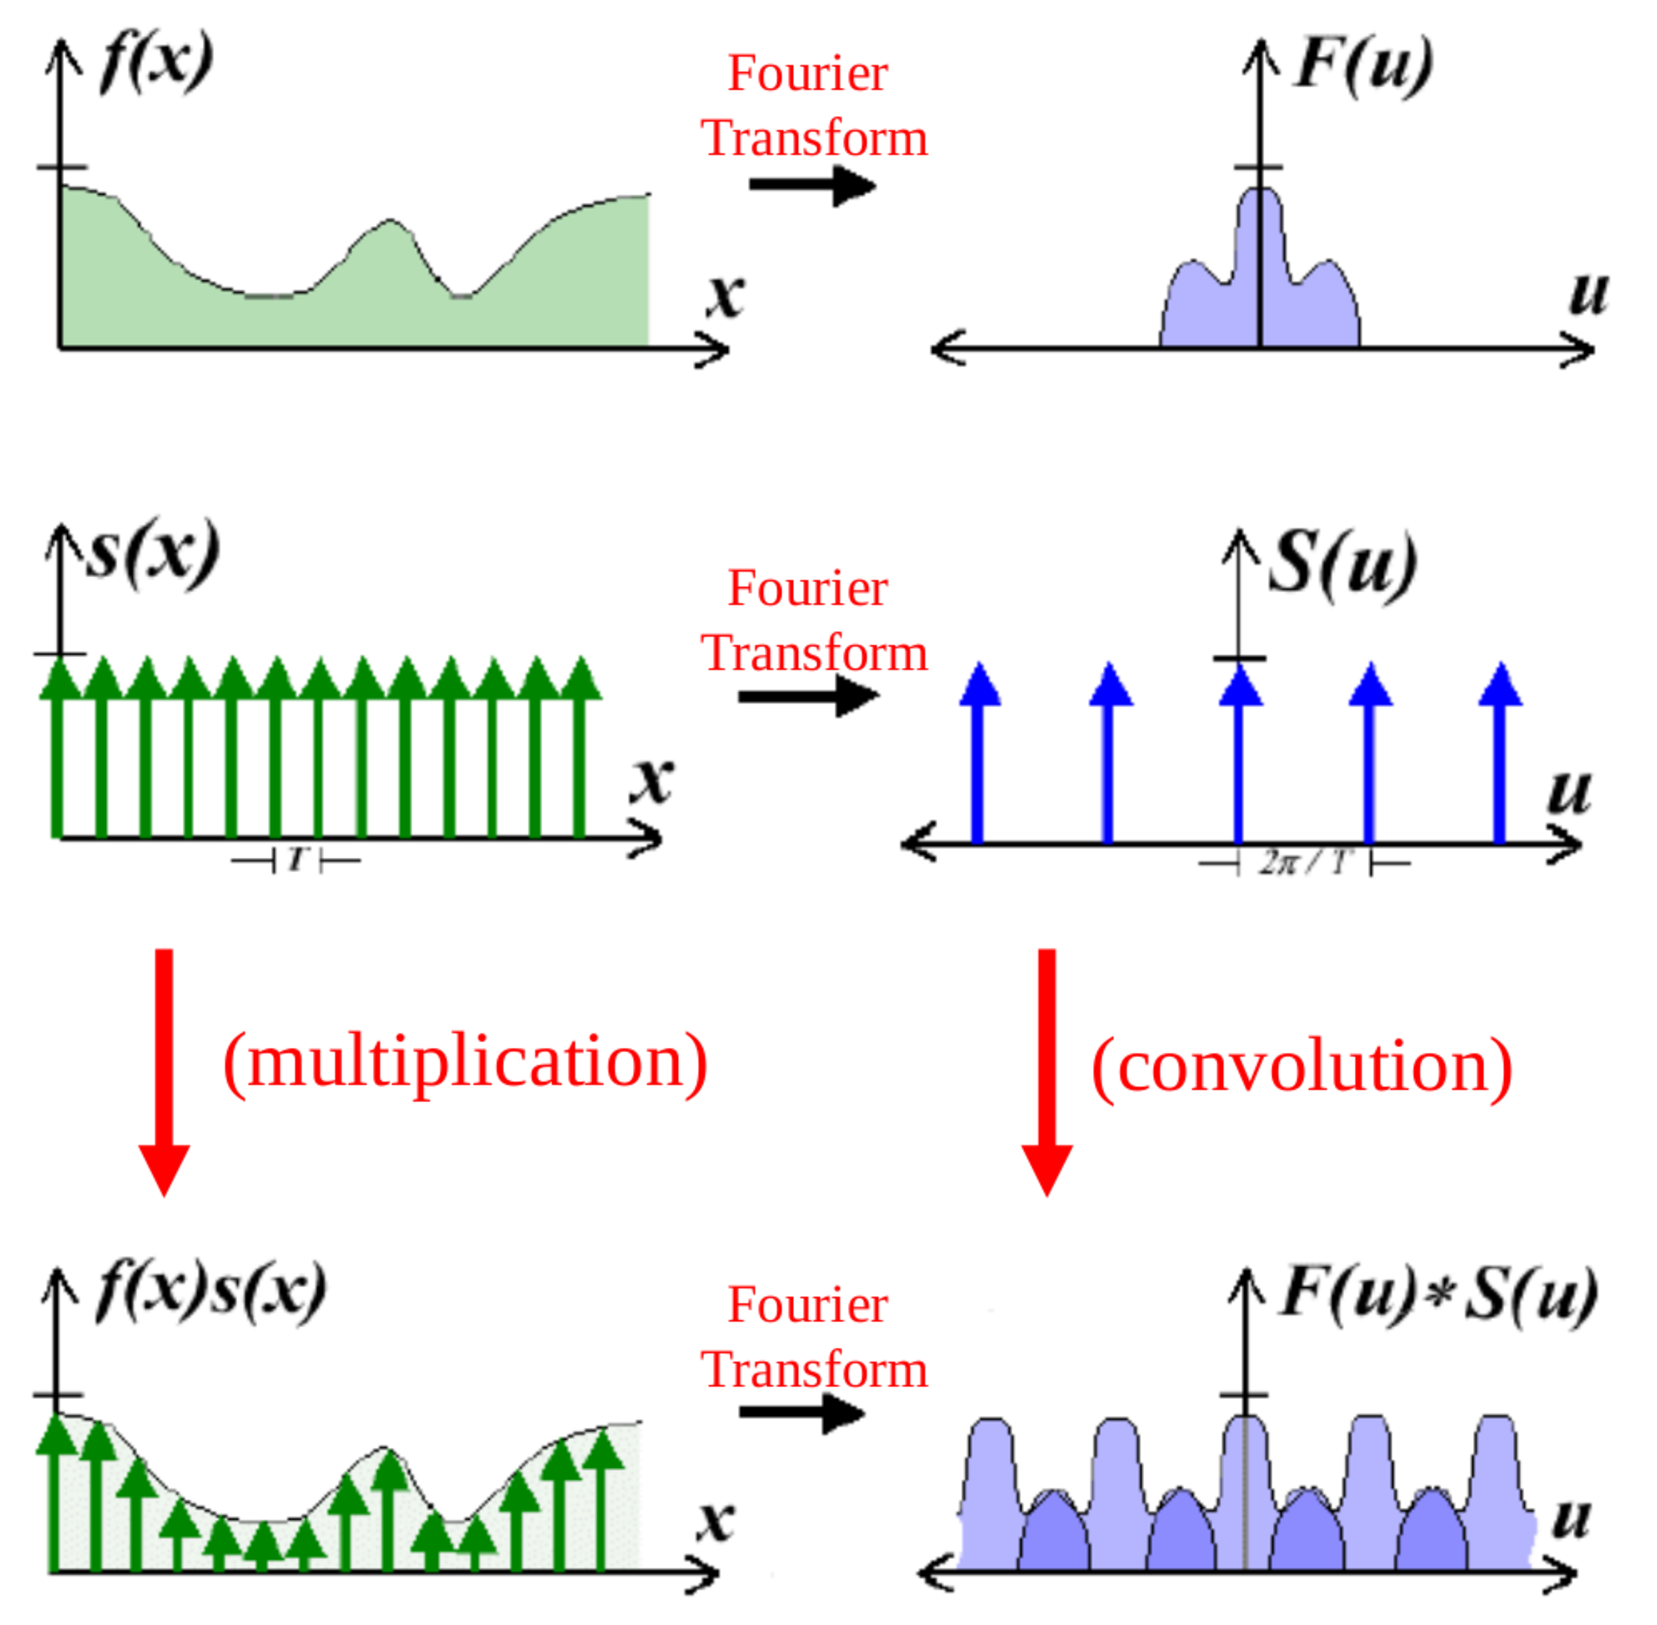
\includegraphics[width=0.7\textheight]{fourier.pdf}
			\caption{\footnotesize Faltung, Abtastung und Diskretisierung. Quelle\cite{mit}}
		\end{figure}
	\end{frame}

	\begin{frame}{2D Abtasttheorem}
	\begin{itemize}
		\item Ist das Bildspektrum ausgedehnt, so überlappen sich die sich periodisch wiederholenden Kopien.
		\item Wir können nicht unterscheiden, ob die spektralen Amplituden aus dem Originalspektrum im Zentrum oder von einer der Kopien stammen.
		\item  Um Verzerrungen zu vermeiden, müssen wir Überlappungen ausschließen.
	\end{itemize}
	\end{frame}

	\begin{frame}{2D Abtasttheorem}
	\begin{itemize}
		\item Wir müssen das Spektrum auf den Bereich um den zentralen Punkt des reziproken Gitters bis zu den Linien, die den Zentralgitterpunkt von allen anderen Gitterpunkten trennen, beschränken.
	\end{itemize}
	\begin{figure}
		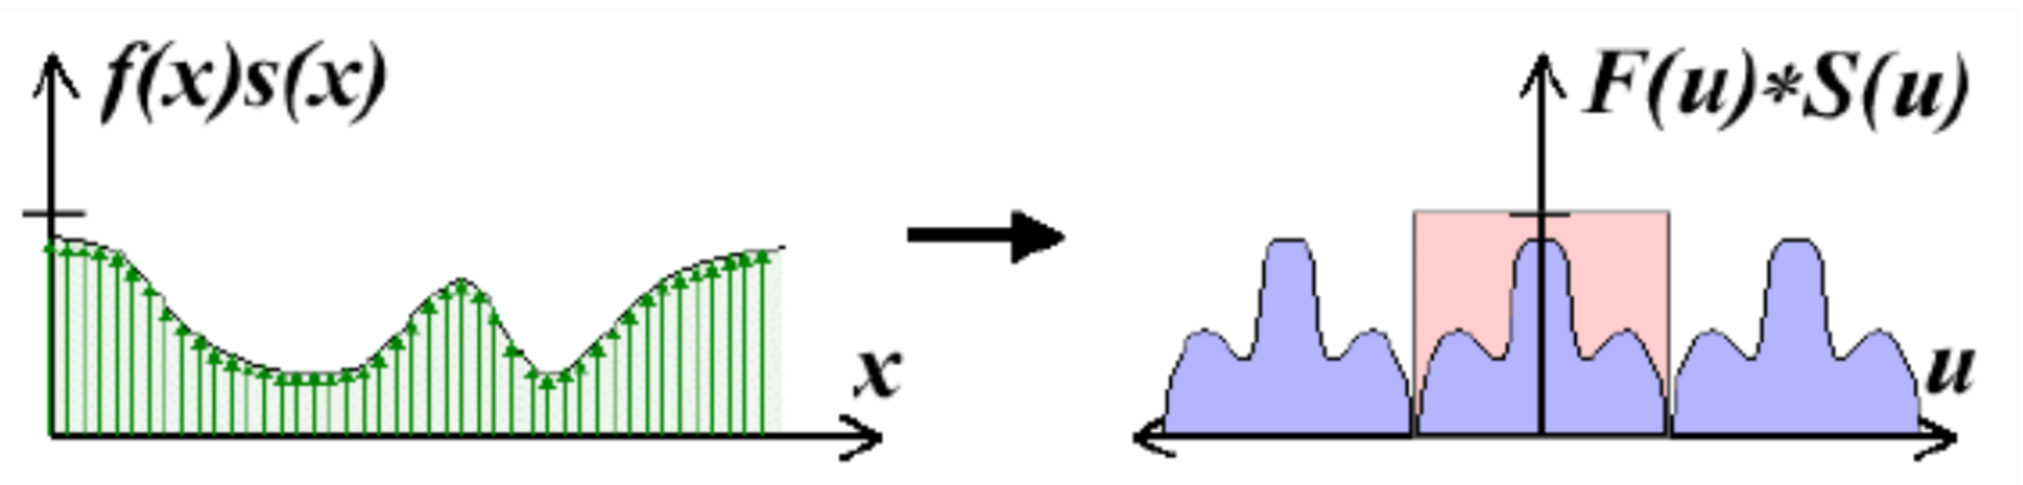
\includegraphics[width=1.3\textheight]{increase.pdf}
		\caption{\footnotesize Beschränkung des Spektrums. Quelle\cite{mit}}
	\end{figure}
	\end{frame}

	\begin{frame}{2D Abtasttheorem}
	\begin{itemize}
		\item Auf einem Rechteckgitter ergibt sich daraus die Bedingung, dass die maximale Wellenzahl, bei der das Bildspektrum nicht null ist,
		auf weniger als die Hälfte des Abstands zwischen den Gitterpunkten in der Bildebene beschränkt werden muss.
		\item Quantitativ kann das so ausgedrückt werden: Ist das Spektrum $\tilde{g}(\kappa)$ einer kontinuierlichen Funktion $g(x)$ bandbegrenzt, d. h.
		$$\tilde{g}(\kappa) = 0 \hspace{1em} \forall \left\|k_{x_1,x_2}\right\|\ge \frac{\Delta k_{x_1,x_2}}{2} $$
		dann kann es aus Punkten welche mit der Schrittweite
		$$\Delta x_{x_1,x_2} = \frac{1}{\Delta k_{x_1,x_2}} $$
		abgetastet wurde exakt rekonstruiert werden.\cite{bildverarbeitung}
	\end{itemize}
	\end{frame}

	\begin{frame}{2D Abtasttheorem}
	\begin{itemize}
		\item Wir erhalten nur dann eine korrekte periodische
		Struktur, wenn wir pro Wellenlänge mindestens zwei Abtastpunkte setzen.
		\item Die maximale Wellenzahl, die ohne Fehler abgetastet werden kann, wird als	Nyquist-Wellenzahl oder Grenzwellenzahl bezeichnet.
	\end{itemize}
	\end{frame}

	\begin{frame}{Realisierung}
	\section{Realisierung}	
	\framesubtitle{Implementierung in MATLAB}
	Ziel: Wie muss ich ein gegebenes Bild abtasten, um noch alle Informationen zu behalten?
	\begin{itemize}
		\item Berechnung der 2D-Fourier-Transformation mittels $fft2$
		\item Bestimmung des \dq Schwellwertes\dq, ab dem wir den Wert der Fouriertransformierten als null annehmen: $Z = max(FFT)*0.001$	
	\end{itemize}

	\end{frame}

	\begin{frame}{Realisierung}
	\framesubtitle{Implementierung in MATLAB}
	\begin{itemize}
	\item Iteration über die Fouriertransformierte, Bestimmung von Grenzfrequenzen $k_x$ und $k_y$ durch Vergleich mit $Z$
	\item Bestimmung der Abtastdistanz: $d_x\leq \frac{1}{2k_x}*I_{Breite}$
	\item Abtastung des Orginalbildes in der Distanz $d_x$ bzw. $d_y$, jeweils mittig
	\item Anzeige des abgetasteten Bildes
	\end{itemize}
	Berechnung Vgl. \cite{dip}
	\end{frame}
	
		\begin{frame}{Realisierung}
	\framesubtitle{MATLAB: FFT2}
	Unser Programm verwendet die matlab-interne fft2-Funktion:
	$$Y_{p+1,q+1} = \sum_{j=0}^{m-1}\sum_{k=0}^{n-1}e^{-2\pi i(\frac{jp}{m}+\frac{kq}{n})}X_{j+1,k+1}$$ mit $X$: Matrix im Ortsraum ($m\times n$), $p,j: 0 - m-1$, $q,k: 0 - n-1$
	
	$Y$ ist ebenfalls eine ($m\times n$)-Matrix
	
	Vgl. \cite{fft2}
	\end{frame}
	\begin{frame}{Realisierung}
	\framesubtitle{MATLAB: FFT2}
	Vgl. DFT aus der Vorlesung
	
	Unterschiedlich: Normierung, Division durch $m$ bzw. $n$
	
	$$ e^{-2\pi i(\frac{jp}{m}+\frac{kq}{n})} $$ vs. 
	$$ e^{-i(jp+kq)} $$
	
	Wichtig für das $\Delta_x / \Delta_y$-Kriterium
	\end{frame}
	
	\begin{frame}{Realisierung}
	Demo
	\end{frame}
	\begin{frame}{Fazit}
	\section{Fazit}
	\begin{itemize}
		\item Faustregel: Je größer die Frequenzen, desto niedriger die Sampledistanz
		\item Fouriertransformation zeigt Verteilung, und ermöglicht die Abschätzung
		\item Praktische Anwendung: Kompression
	\end{itemize}
	\end{frame}
	
	\begin{frame}{Quellen}
		\begin{multicols}{2}
		\tiny{
			\bibliographystyle{plainnat}
			\bibliography{literatur}
		}
		\end{multicols}
	\end{frame}
	
\end{document}